% =====================================================================
% preview_fig02_pareto_mix_a_primary -- R/ggplot2 -> tikzDevice (Frame-A, ESWA target)
% Canonical-JSON-only. Regenerate: Rscript submissions/frame-a-eswa/figures-r/make_figures_frame_a.R
% Provenance (JSON path :: field = plotted value), one line per series:
% SOURCE: results/frame_a/cells/cell_llama-3.2-1b_real_MIX_A_both_s*.json :: mean(quality.Q), mean(cost.total_gpu_s) = n=3 Q=0.9383 cost=224.08
% SOURCE: results/frame_a/cells/cell_llama-3.2-1b_real_MIX_A_cost_only_s*.json :: mean(quality.Q), mean(cost.total_gpu_s) = n=3 Q=0.7838 cost=1845.93
% SOURCE: results/frame_a/cells/cell_llama-3.2-1b_real_MIX_A_damage_only_s*.json :: mean(quality.Q), mean(cost.total_gpu_s) = n=3 Q=0.9383 cost=224.29
% SOURCE: results/frame_a/cells/cell_llama-3.2-1b_real_MIX_A_oracle_s*.json :: mean(quality.Q), mean(cost.total_gpu_s) = n=3 Q=0.7496 cost=154.69
% SOURCE: results/frame_a/cells/cell_llama-3.2-1b_real_MIX_A_always_edit_s*.json :: mean(quality.Q), mean(cost.total_gpu_s) = n=3 Q=0.8266 cost=225.43
% SOURCE: results/frame_a/cells/cell_llama-3.2-1b_real_MIX_A_always_grace_s*.json :: mean(quality.Q), mean(cost.total_gpu_s) = n=3 Q=0.9544 cost=229.01
% SOURCE: results/frame_a/cells/cell_llama-3.2-1b_real_MIX_A_always_rag_s*.json :: mean(quality.Q), mean(cost.total_gpu_s) = n=3 Q=0.6040 cost=186.58
% SOURCE: results/frame_a/cells/cell_llama-3.2-1b_real_MIX_A_always_ft_s*.json :: mean(quality.Q), mean(cost.total_gpu_s) = n=3 Q=0.6786 cost=5.60
% SOURCE: results/frame_a/cells/cell_llama-3.2-1b_real_MIX_A_always_reject_s*.json :: mean(quality.Q), mean(cost.total_gpu_s) = n=3 Q=0.3000 cost=5.90
% SOURCE: results/frame_a/cells/cell_llama-3.2-1b_real_MIX_A_random_s*.json :: mean(quality.Q), mean(cost.total_gpu_s) = n=3 Q=0.8279 cost=963.13
% SOURCE: results/frame_a/cells/cell_llama-3.2-1b_real_MIX_A_ft_merge_s*.json :: mean(quality.Q), mean(cost.total_gpu_s) = n=3 Q=0.6786 cost=637.06
% SOURCE: results/frame_a/cells/cell_llama-3.2-1b_real_MIX_B_both_s*.json :: mean(quality.Q), mean(cost.total_gpu_s) = n=2 Q=0.8857 cost=216.68
% SOURCE: results/frame_a/cells/cell_llama-3.2-1b_real_MIX_B_cost_only_s*.json :: mean(quality.Q), mean(cost.total_gpu_s) = n=2 Q=0.8150 cost=191.97
% SOURCE: results/frame_a/cells/cell_llama-3.2-1b_real_MIX_B_damage_only_s*.json :: mean(quality.Q), mean(cost.total_gpu_s) = n=2 Q=0.8857 cost=216.79
% SOURCE: results/frame_a/cells/cell_llama-3.2-1b_real_MIX_B_oracle_s*.json :: mean(quality.Q), mean(cost.total_gpu_s) = n=2 Q=0.7328 cost=155.65
% SOURCE: results/frame_a/cells/cell_llama-3.2-1b_real_MIX_B_always_edit_s*.json :: mean(quality.Q), mean(cost.total_gpu_s) = n=2 Q=0.8383 cost=208.45
% SOURCE: results/frame_a/cells/cell_llama-3.2-1b_real_MIX_B_always_grace_s*.json :: mean(quality.Q), mean(cost.total_gpu_s) = n=2 Q=0.8912 cost=224.21
% SOURCE: results/frame_a/cells/cell_llama-3.2-1b_real_MIX_B_always_rag_s*.json :: mean(quality.Q), mean(cost.total_gpu_s) = n=2 Q=0.6048 cost=226.14
% SOURCE: results/frame_a/cells/cell_llama-3.2-1b_real_MIX_B_always_ft_s*.json :: mean(quality.Q), mean(cost.total_gpu_s) = n=1 Q=0.2920 cost=6.22
% SOURCE: results/frame_a/cells/cell_llama-3.2-1b_real_MIX_B_always_reject_s*.json :: mean(quality.Q), mean(cost.total_gpu_s) = n=1 Q=0.3000 cost=5.99
% SOURCE: results/frame_a/cells/cell_llama-3.2-1b_real_MIX_B_random_s*.json :: mean(quality.Q), mean(cost.total_gpu_s) = n=1 Q=0.7998 cost=88.25
% SOURCE: results/frame_a/cells/cell_llama-3.2-1b_real_MIX_B_ft_merge_s*.json :: mean(quality.Q), mean(cost.total_gpu_s) = n=1 Q=0.8716 cost=7.36
% =====================================================================
% WARNING: QA-PREVIEW-NOT-FOR-SUBMISSION (generated 2026-07-23 08:37:24 EDT)
% This file is NOT camera-ready. The MIX_A preview under figures-qa/
% !TEX encoding = UTF-8 Unicode
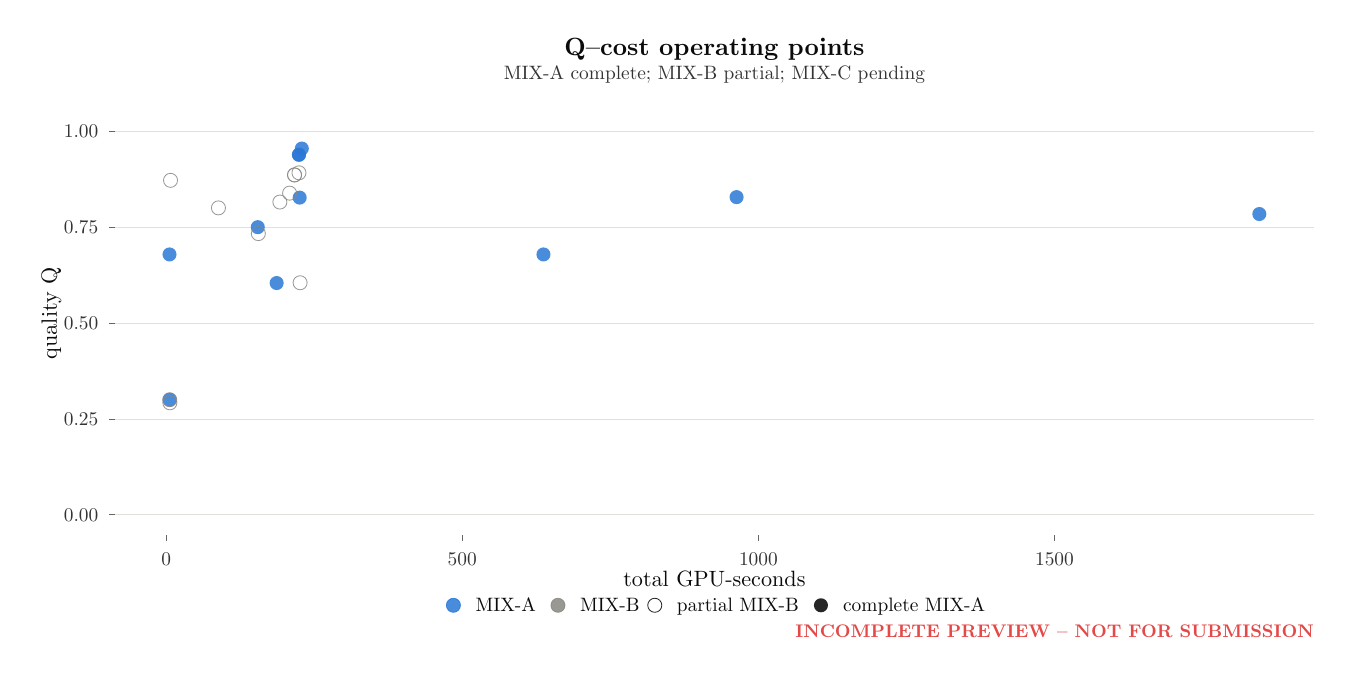
\begin{tikzpicture}[x=1pt,y=1pt]
\definecolor{fillColor}{RGB}{255,255,255}
\path[use as bounding box,fill=fillColor,fill opacity=0.00] (0,0) rectangle (469.75,227.65);
\begin{scope}
\path[clip] (  0.00,  0.00) rectangle (469.75,227.65);
\definecolor{fillColor}{RGB}{255,255,255}

\path[fill=fillColor] (  0.00,  0.00) rectangle (469.76,227.65);
\end{scope}
\begin{scope}
\path[clip] ( 31.56, 44.32) rectangle (464.75,204.51);
\definecolor{drawColor}{RGB}{225,224,217}

\path[draw=drawColor,line width= 0.3pt,line join=round] ( 31.56, 51.60) --
	(464.75, 51.60);

\path[draw=drawColor,line width= 0.3pt,line join=round] ( 31.56, 86.27) --
	(464.75, 86.27);

\path[draw=drawColor,line width= 0.3pt,line join=round] ( 31.56,120.94) --
	(464.75,120.94);

\path[draw=drawColor,line width= 0.3pt,line join=round] ( 31.56,155.62) --
	(464.75,155.62);

\path[draw=drawColor,line width= 0.3pt,line join=round] ( 31.56,190.29) --
	(464.75,190.29);
\definecolor{fillColor}{RGB}{42,120,214}

\path[fill=fillColor,fill opacity=0.85] ( 98.00,181.73) circle (  2.54);

\path[fill=fillColor,fill opacity=0.85] (445.06,160.31) circle (  2.54);

\path[fill=fillColor,fill opacity=0.85] ( 98.05,181.73) circle (  2.54);

\path[fill=fillColor,fill opacity=0.85] ( 83.15,155.56) circle (  2.54);

\path[fill=fillColor,fill opacity=0.85] ( 98.29,166.24) circle (  2.54);

\path[fill=fillColor,fill opacity=0.85] ( 99.06,183.97) circle (  2.54);

\path[fill=fillColor,fill opacity=0.85] ( 89.97,135.37) circle (  2.54);

\path[fill=fillColor,fill opacity=0.85] ( 51.25,145.71) circle (  2.54);

\path[fill=fillColor,fill opacity=0.85] ( 51.31, 93.21) circle (  2.54);

\path[fill=fillColor,fill opacity=0.85] (256.15,166.42) circle (  2.54);

\path[fill=fillColor,fill opacity=0.85] (186.38,145.71) circle (  2.54);
\definecolor{drawColor}{RGB}{137,135,129}

\path[draw=drawColor,draw opacity=0.85,line width= 0.3pt,line join=round,line cap=round] ( 96.42,174.44) circle (  2.54);

\path[draw=drawColor,draw opacity=0.85,line width= 0.3pt,line join=round,line cap=round] ( 91.13,164.63) circle (  2.54);

\path[draw=drawColor,draw opacity=0.85,line width= 0.3pt,line join=round,line cap=round] ( 96.44,174.44) circle (  2.54);

\path[draw=drawColor,draw opacity=0.85,line width= 0.3pt,line join=round,line cap=round] ( 83.36,153.23) circle (  2.54);

\path[draw=drawColor,draw opacity=0.85,line width= 0.3pt,line join=round,line cap=round] ( 94.65,167.86) circle (  2.54);

\path[draw=drawColor,draw opacity=0.85,line width= 0.3pt,line join=round,line cap=round] ( 98.03,175.20) circle (  2.54);

\path[draw=drawColor,draw opacity=0.85,line width= 0.3pt,line join=round,line cap=round] ( 98.44,135.48) circle (  2.54);

\path[draw=drawColor,draw opacity=0.85,line width= 0.3pt,line join=round,line cap=round] ( 51.38, 92.09) circle (  2.54);

\path[draw=drawColor,draw opacity=0.85,line width= 0.3pt,line join=round,line cap=round] ( 51.33, 93.21) circle (  2.54);

\path[draw=drawColor,draw opacity=0.85,line width= 0.3pt,line join=round,line cap=round] ( 68.93,162.52) circle (  2.54);

\path[draw=drawColor,draw opacity=0.85,line width= 0.3pt,line join=round,line cap=round] ( 51.62,172.48) circle (  2.54);
\end{scope}
\begin{scope}
\path[clip] (  0.00,  0.00) rectangle (469.75,227.65);
\definecolor{drawColor}{gray}{0.20}

\node[text=drawColor,anchor=base east,inner sep=0pt, outer sep=0pt, scale=  0.70] at ( 25.51, 49.19) {0.00};

\node[text=drawColor,anchor=base east,inner sep=0pt, outer sep=0pt, scale=  0.70] at ( 25.51, 83.86) {0.25};

\node[text=drawColor,anchor=base east,inner sep=0pt, outer sep=0pt, scale=  0.70] at ( 25.51,118.53) {0.50};

\node[text=drawColor,anchor=base east,inner sep=0pt, outer sep=0pt, scale=  0.70] at ( 25.51,153.21) {0.75};

\node[text=drawColor,anchor=base east,inner sep=0pt, outer sep=0pt, scale=  0.70] at ( 25.51,187.88) {1.00};
\end{scope}
\begin{scope}
\path[clip] (  0.00,  0.00) rectangle (469.75,227.65);
\definecolor{drawColor}{gray}{0.40}

\path[draw=drawColor,line width= 0.3pt,line join=round] ( 29.56, 51.60) --
	( 31.56, 51.60);

\path[draw=drawColor,line width= 0.3pt,line join=round] ( 29.56, 86.27) --
	( 31.56, 86.27);

\path[draw=drawColor,line width= 0.3pt,line join=round] ( 29.56,120.94) --
	( 31.56,120.94);

\path[draw=drawColor,line width= 0.3pt,line join=round] ( 29.56,155.62) --
	( 31.56,155.62);

\path[draw=drawColor,line width= 0.3pt,line join=round] ( 29.56,190.29) --
	( 31.56,190.29);
\end{scope}
\begin{scope}
\path[clip] (  0.00,  0.00) rectangle (469.75,227.65);
\definecolor{drawColor}{gray}{0.40}

\path[draw=drawColor,line width= 0.3pt,line join=round] ( 50.05, 42.32) --
	( 50.05, 44.32);

\path[draw=drawColor,line width= 0.3pt,line join=round] (157.04, 42.32) --
	(157.04, 44.32);

\path[draw=drawColor,line width= 0.3pt,line join=round] (264.04, 42.32) --
	(264.04, 44.32);

\path[draw=drawColor,line width= 0.3pt,line join=round] (371.04, 42.32) --
	(371.04, 44.32);
\end{scope}
\begin{scope}
\path[clip] (  0.00,  0.00) rectangle (469.75,227.65);
\definecolor{drawColor}{gray}{0.20}

\node[text=drawColor,anchor=base,inner sep=0pt, outer sep=0pt, scale=  0.70] at ( 50.05, 33.45) {0};

\node[text=drawColor,anchor=base,inner sep=0pt, outer sep=0pt, scale=  0.70] at (157.04, 33.45) {500};

\node[text=drawColor,anchor=base,inner sep=0pt, outer sep=0pt, scale=  0.70] at (264.04, 33.45) {1000};

\node[text=drawColor,anchor=base,inner sep=0pt, outer sep=0pt, scale=  0.70] at (371.04, 33.45) {1500};
\end{scope}
\begin{scope}
\path[clip] (  0.00,  0.00) rectangle (469.75,227.65);
\definecolor{drawColor}{RGB}{11,11,11}

\node[text=drawColor,anchor=base,inner sep=0pt, outer sep=0pt, scale=  0.80] at (248.16, 25.57) {total GPU-seconds};
\end{scope}
\begin{scope}
\path[clip] (  0.00,  0.00) rectangle (469.75,227.65);
\definecolor{drawColor}{RGB}{11,11,11}

\node[text=drawColor,rotate= 90.00,anchor=base,inner sep=0pt, outer sep=0pt, scale=  0.80] at ( 10.51,124.41) {quality Q};
\end{scope}
\begin{scope}
\path[clip] (  0.00,  0.00) rectangle (469.75,227.65);
\definecolor{drawColor}{RGB}{42,120,214}
\definecolor{fillColor}{RGB}{42,120,214}

\path[draw=drawColor,draw opacity=0.85,line width= 0.3pt,line join=round,line cap=round,fill=fillColor,fill opacity=0.85] (153.84, 18.93) circle (  2.54);
\end{scope}
\begin{scope}
\path[clip] (  0.00,  0.00) rectangle (469.75,227.65);
\definecolor{drawColor}{RGB}{137,135,129}
\definecolor{fillColor}{RGB}{137,135,129}

\path[draw=drawColor,draw opacity=0.85,line width= 0.3pt,line join=round,line cap=round,fill=fillColor,fill opacity=0.85] (191.62, 18.93) circle (  2.54);
\end{scope}
\begin{scope}
\path[clip] (  0.00,  0.00) rectangle (469.75,227.65);
\definecolor{drawColor}{RGB}{11,11,11}

\node[text=drawColor,anchor=base west,inner sep=0pt, outer sep=0pt, scale=  0.70] at (161.84, 16.52) {MIX-A};
\end{scope}
\begin{scope}
\path[clip] (  0.00,  0.00) rectangle (469.75,227.65);
\definecolor{drawColor}{RGB}{11,11,11}

\node[text=drawColor,anchor=base west,inner sep=0pt, outer sep=0pt, scale=  0.70] at (199.62, 16.52) {MIX-B};
\end{scope}
\begin{scope}
\path[clip] (  0.00,  0.00) rectangle (469.75,227.65);
\definecolor{drawColor}{RGB}{0,0,0}

\path[draw=drawColor,draw opacity=0.85,line width= 0.3pt,line join=round,line cap=round] (226.60, 18.93) circle (  2.54);
\end{scope}
\begin{scope}
\path[clip] (  0.00,  0.00) rectangle (469.75,227.65);
\definecolor{fillColor}{RGB}{0,0,0}

\path[fill=fillColor,fill opacity=0.85] (286.65, 18.93) circle (  2.54);
\end{scope}
\begin{scope}
\path[clip] (  0.00,  0.00) rectangle (469.75,227.65);
\definecolor{drawColor}{RGB}{11,11,11}

\node[text=drawColor,anchor=base west,inner sep=0pt, outer sep=0pt, scale=  0.70] at (234.60, 16.52) {partial MIX-B};
\end{scope}
\begin{scope}
\path[clip] (  0.00,  0.00) rectangle (469.75,227.65);
\definecolor{drawColor}{RGB}{11,11,11}

\node[text=drawColor,anchor=base west,inner sep=0pt, outer sep=0pt, scale=  0.70] at (294.65, 16.52) {complete MIX-A};
\end{scope}
\begin{scope}
\path[clip] (  0.00,  0.00) rectangle (469.75,227.65);
\definecolor{drawColor}{gray}{0.20}

\node[text=drawColor,anchor=base,inner sep=0pt, outer sep=0pt, scale=  0.70] at (248.16,208.87) {MIX-A complete; MIX-B partial; MIX-C pending};
\end{scope}
\begin{scope}
\path[clip] (  0.00,  0.00) rectangle (469.75,227.65);
\definecolor{drawColor}{RGB}{11,11,11}

\node[text=drawColor,anchor=base,inner sep=0pt, outer sep=0pt, scale=  0.90] at (248.16,217.44) {\bfseries Q--cost operating points};
\end{scope}
\begin{scope}
\path[clip] (  0.00,  0.00) rectangle (469.75,227.65);
\definecolor{drawColor}{RGB}{227,73,72}

\node[text=drawColor,anchor=base east,inner sep=0pt, outer sep=0pt, scale=  0.66] at (464.75,  7.28) {\bfseries INCOMPLETE PREVIEW -- NOT FOR SUBMISSION};
\end{scope}
\end{tikzpicture}
